\subsubsection{Почему транзисторные ключи с инжекционным питанием имеют источник питания с самой маленькой ЭДС среди всех ключей? Какой?}

Ключ на интегрально-инжекторной логике представляет собой ключ, где в отличие от простого эмиттерного ключа резисторы (в частности Rб и Rк) заменены на генераторы стабильного тока, при этом все транзисторы могут быть запитаны от одного источника ЭДС с использованием горизонтального многоколлекторного транзистора.

Поясним сказанное на примере.

\begin{center}
	\begin{figure}[h!]
		\center{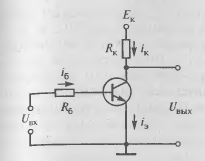
\includegraphics[scale=3]{iil/image001.png}}
		\caption{Простейший ключ}	
		\label{iil1}
	\end{figure}
\end{center}

 

\begin{center}
	\begin{figure}[h!]
		\center{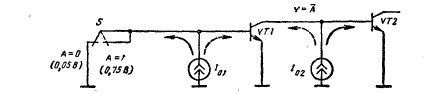
\includegraphics[scale=2]{iil/image003.png}}
		\caption{Инвертор на базе иил ключа}	
		\label{iil3}
	\end{figure}
\end{center}



В иил ключе не используются резисторы Rб и Rк, тратящие много времени и мощности. 

Вместо них используются источники питания. 

В левом положении ключа S, соответствующем уровню  лог. 0 (0.05 В) ток от генератора идет через ключ (транзистор , выполняющий роль ключа, аналогичный транзисторам VT1 и VT2) на землю. При этом транзистор VT1 заперт, потому что на его базу не подано напряжение, достаточное для отпирания ключа. Поэтому ток от генератора I2 идет на базу транзистора VT2 и переводит его в режим насыщения. Напряжение база-эмиттер такого транзистора около 0.75 В, что соответствует уровню лог. 1. Выходной сигнал можно снять с клеммы Y.

В правом положении ключа S ток I1 отпирает транзистор VT1, переводя его в режим насыщения. Условие такого перехода -- Biб$>$Iкнас выполнено. На схеме BI1$>$I2. При I1=I2 и B $>$ 1 это всегда выполняется. Напряжение между коллекторам и эмиттером выбранного насыщенного транзистора, как уже было сказано, 0.05 В. На клемме Y -- искомый нулевой сигнал.

В иил используются источники питания с самой низкой эдс среди всех ключей, потому что транзистор переходит в насыщение уже при напряжении Uбэ=0.75В. Резистор используется один -- в источнике питания, для его стабилизации. Поэтому, ЭДС источника -- около 1,15В. В других ключах необходимо большее эдс, потому что значительная часть напряжения теряется на Rб.

В частности, источник подключается так:

\begin{center}
	\begin{figure}[h!]
		\center{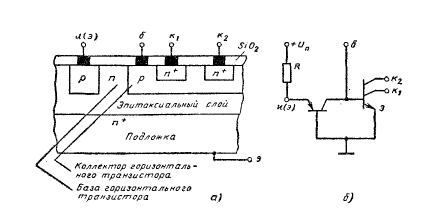
\includegraphics[scale=1.5]{iil/image005.png}}
		\caption{}	
		\label{iil5}
	\end{figure}
\end{center}



Применение:
\begin{center}
	\begin{figure}[h!]
		\center{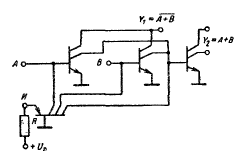
\includegraphics[scale=2]{iil/image007.png}}
		\caption{}	
		\label{iil7}
	\end{figure}
\end{center}

На этой схеме и схеме б) показано, что для запитывания иил ключа достаточно подключить источник эдс через резистор R к горизонтальному pnp транзистору. Он выдает на своем коллекторе (коллекторах) стабильный ток, от которых можно подать питание все имеющиеся в ней npn транзисторы, необходимое для их отпирания (насыщения) или запирания (перевода в режим отсечки).

\subsubsection{Какие требования предъявляются по коэффициенту усиления к транзисторам ключей ИИЛ и почему такие?}

Ключ на интегрально-инжекторной логике представляет собой ключ, где в отличие от простого эмиттерного ключа резисторы (в частности Rб и Rк) заменены на генераторы стабильного тока, при этом все транзисторы могут быть запитаны от одного источника ЭДС с использованием горизонтального многоколлекторного транзистора.

Поясним сказанное на примере.

\begin{center}
	\begin{figure}[h!]
		\center{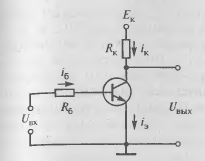
\includegraphics[scale=3]{iil/image001.png}}
		\caption{Простейший ключ}	
		\label{iil1}
	\end{figure}
\end{center}

 

\begin{center}
	\begin{figure}[h!]
		\center{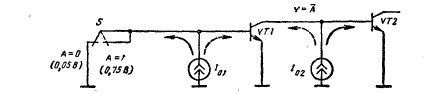
\includegraphics[scale=2]{iil/image003.png}}
		\caption{Инвертор на базе иил ключа}	
		\label{iil3}
	\end{figure}
\end{center}



В иил ключе не используются резисторы Rб и Rк, тратящие много времени и мощности. 

Вместо них используются источники питания. 

В левом положении ключа S, соответствующем уровню  лог. 0 (0.05 В) ток от генератора идет через ключ (транзистор , выполняющий роль ключа, аналогичный транзисторам VT1 и VT2) на землю. При этом транзистор VT1 заперт, потому что на его базу не подано напряжение, достаточное для отпирания ключа. Поэтому ток от генератора I2 идет на базу транзистора VT2 и переводит его в режим насыщения. Напряжение база-эмиттер такого транзистора около 0.75 В, что соответствует уровню лог. 1. Выходной сигнал можно снять с клеммы Y.

В правом положении ключа S ток I1 отпирает транзистор VT1, переводя его в режим насыщения. Условие такого перехода -- Biб$>$Iкнас выполнено. На схеме BI1$>$I2. При I1=I2 и B $>$ 1 это всегда выполняется. Напряжение между коллекторам и эмиттером выбранного насыщенного транзистора, как уже было сказано, 0.05 В. На клемме Y -- искомый нулевой сигнал.

Именно поэтому при использовании генераторов стабильного тока с одинаковой силой тока, для обеспечения включения ключа и его выключения, то есть перевода транзисторов VT1 и VT2 в режим насыщения коэффициент усиления по току B для транзисторов должен быть таким, чтобы выполнялось условие BI1$>$I2, то есть B больше 1. Поэтому можно использовать многоколлекторные транзисторы, которые способствуют миниатюризации логической схемы, обладая как правило низким B.

\subsubsection{В каких областях может находиться РТ транзисторов ИИЛ-ключей?}

Ключ на интегрально-инжекторной логике представляет собой ключ, где в отличие от простого эмиттерного ключа резисторы (в частности Rб и Rк) заменены на генераторы стабильного тока, при этом все транзисторы могут быть запитаны от одного источника ЭДС с использованием горизонтального многоколлекторного транзистора.

Поясним сказанное на примере.

\begin{center}
	\begin{figure}[h!]
		\center{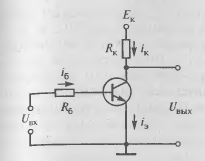
\includegraphics[scale=3]{iil/image001.png}}
		\caption{Простейший ключ}	
		\label{iil1}
	\end{figure}
\end{center}

 

\begin{center}
	\begin{figure}[h!]
		\center{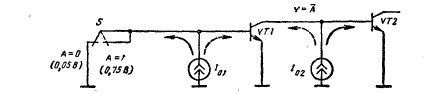
\includegraphics[scale=2]{iil/image003.png}}
		\caption{Инвертор на базе иил ключа}	
		\label{iil3}
	\end{figure}
\end{center}



В иил ключе не используются резисторы Rб и Rк, тратящие много времени и мощности. 

Вместо них используются источники питания. 

В левом положении ключа S, соответствующем уровню  лог. 0 (0.05 В) ток от генератора идет через ключ (транзистор , выполняющий роль ключа, аналогичный транзисторам VT1 и VT2) на землю. При этом транзистор VT1 заперт, потому что на его базу не подано напряжение, достаточное для отпирания ключа. Поэтому ток от генератора I2 идет на базу транзистора VT2 и переводит его в режим насыщения. Напряжение база-эмиттер такого транзистора около 0.75 В, что соответствует уровню лог. 1. Выходной сигнал можно снять с клеммы Y.

В правом положении ключа S ток I1 отпирает транзистор VT1, переводя его в режим насыщения. Условие такого перехода -- Biб$>$Iкнас выполнено. На схеме BI1$>$I2. При I1=I2 и B $>$ 1 это всегда выполняется. Напряжение между коллекторам и эмиттером выбранного насыщенного транзистора, как уже было сказано, 0.05 В. На клемме Y -- искомый нулевой сигнал.

Вывод: при подаче на эмиттерный переход транзистора напряжение, соответствующее уровню лог. нуля, транзистор VT1 находится в режиме отсечки, потому что базовый ток пренебрежимо мал и двигаясь по линии нагрузки по кривым выходных характеристик транзистора мы попадем в область отсечки. Транзистор VT2 находится в режиме насыщения.

При подаче на эмиттерный переход напряжения, соответствующего уровню лог. единицы, транзистор VT1 находится в режиме насыщения, потому что BI1$>$I2, а транзистор VT2 -- в режиме отсечки.

Значит, транзисторы VT1 и VT2 в схеме на ИИЛ ключе могут находиться в режимах отсечки и насыщения.Вывод: при подаче на эмиттерный переход транзистора напряжение, соответствующее уровню лог. нуля, транзистор VT1 находится в режиме отсечки, потому что базовый ток пренебрежимо мал и двигаясь по линии нагрузки по кривым выходных характеристик транзистора мы попадем в область отсечки. Транзистор VT2 находится в режиме насыщения.

\subsubsection{Почему микросхемы на ИИЛ-ключах занимают очень маленькую площадь на подложке?}

Ключ на интегрально-инжекторной логике представляет собой ключ, где в отличие от простого эмиттерного ключа резисторы (в частности Rб и Rк) заменены на генераторы стабильного тока, при этом все транзисторы могут быть запитаны от одного источника ЭДС с использованием горизонтального многоколлекторного транзистора.

Поясним сказанное на примере.

\begin{center}
	\begin{figure}[h!]
		\center{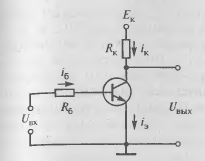
\includegraphics[scale=3]{iil/image001.png}}
		\caption{Простейший ключ}	
		\label{iil1}
	\end{figure}
\end{center}

 

\begin{center}
	\begin{figure}[h!]
		\center{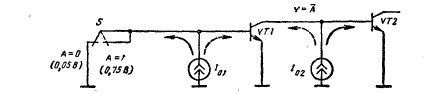
\includegraphics[scale=2]{iil/image003.png}}
		\caption{Инвертор на базе иил ключа}	
		\label{iil3}
	\end{figure}
\end{center}



В иил ключе не используются резисторы Rб и Rк, тратящие много времени и мощности. 

Вместо них используются источники питания. 

В левом положении ключа S, соответствующем уровню  лог. 0 (0.05 В) ток от генератора идет через ключ (транзистор , выполняющий роль ключа, аналогичный транзисторам VT1 и VT2) на землю. При этом транзистор VT1 заперт, потому что на его базу не подано напряжение, достаточное для отпирания ключа. Поэтому ток от генератора I2 идет на базу транзистора VT2 и переводит его в режим насыщения. Напряжение база-эмиттер такого транзистора около 0.75 В, что соответствует уровню лог. 1. Выходной сигнал можно снять с клеммы Y.

В правом положении ключа S ток I1 отпирает транзистор VT1, переводя его в режим насыщения. Условие такого перехода -- Biб$>$Iкнас выполнено. На схеме BI1$>$I2. При I1=I2 и B $>$ 1 это всегда выполняется. Напряжение между коллекторам и эмиттером выбранного насыщенного транзистора, как уже было сказано, 0.05 В. На клемме Y -- искомый нулевой сигнал.

Элементы на иил ключах занимают малую площадь на подложке по следующим причинам:

Во-первых, в самой схеме ключа не используются резисторы, они заменены источниками стабильного тока. В связи с этим, на плате не нужно тратить место на резисторы. 

Во-вторых, используются многоколлекторные транзисторы, которые позволяют запитать всю схему одним источником тока. Один источник тока подключается ко всем транзисторам так:
\begin{center}
	\begin{figure}[h!]
		\center{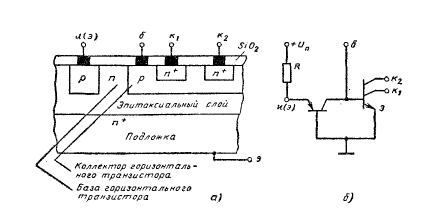
\includegraphics[scale=1.5]{iil/image005.png}}
		\caption{}	
		\label{iil5}
	\end{figure}
\end{center}



\begin{center}
	\begin{figure}[h!]
		\center{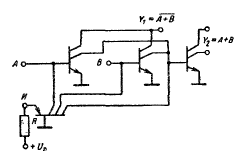
\includegraphics[scale=2]{iil/image007.png}}
		\caption{}	
		\label{iil7}
	\end{figure}
\end{center}
На этой схеме и схеме б) показано, что для запитывания иил ключа достаточно подключить источник эдс через резистор R к горизонтальному pnp транзистору. Он выдает на своем коллекторе (коллекторах) стабильный ток, от которых можно подать питание все имеющиеся в ней npn транзисторы, необходимое для их отпирания (насыщения) или запирания (перевода в режим отсечки).

Таким, образом, схемы на иил ключах занимают мало место на подложке, потому что не используются резисторы (кроме резистора R на схеме б), который обесп. стабил. тока), можно использовать многоколлекторные горизонтальные транзисторы для подачи тока от одного источника ко всем транзисторам и вертикальные многоколлекторные транзисторы для минимизации количества транзисторов в схеме благодаря тому, что несмотря на то, что многоколлекторные транзисторы обладают меньшим коэффициентом передачи по току, требование к коэфициенту B такое, что B$>$1 (это следует из условия насыщения BIб$>$Bik, где Ib равен Iк).
\subsubsection{Чем определяется быстродействие ИИЛ-ключей?}

Ключ на интегрально-инжекторной логике представляет собой ключ, где в отличие от простого эмиттерного ключа резисторы (в частности Rб и Rк) заменены на генераторы стабильного тока, при этом все транзисторы могут быть запитаны от одного источника ЭДС с использованием горизонтального многоколлекторного транзистора.

Поясним сказанное на примере.

\begin{center}
	\begin{figure}[h!]
		\center{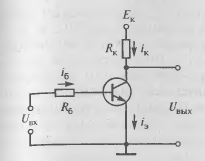
\includegraphics[scale=3]{iil/image001.png}}
		\caption{Простейший ключ}	
		\label{iil1}
	\end{figure}
\end{center}

 

\begin{center}
	\begin{figure}[h!]
		\center{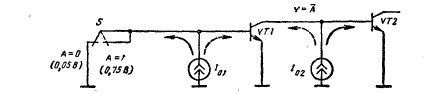
\includegraphics[scale=2]{iil/image003.png}}
		\caption{Инвертор на базе иил ключа}	
		\label{iil3}
	\end{figure}
\end{center}



В иил ключе не используются резисторы Rб и Rк, тратящие много времени и мощности. 

Вместо них используются источники питания. 

\begin{center}
	\begin{figure}[h!]
		\center{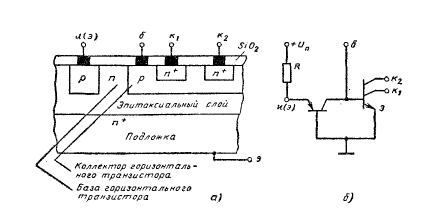
\includegraphics[scale=1.5]{iil/image005.png}}
		\caption{}	
		\label{iil5}
	\end{figure}
\end{center}



\begin{center}
	\begin{figure}[h!]
		\center{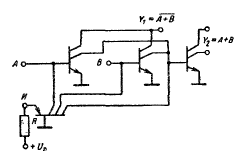
\includegraphics[scale=2]{iil/image007.png}}
		\caption{}	
		\label{iil7}
	\end{figure}
\end{center}
На этой схеме и схеме б) показано, что для запитывания иил ключа достаточно подключить источник эдс через резистор R к горизонтальному pnp транзистору. Он выдает на своем коллекторе (коллекторах) стабильный ток, от которых можно подать питание все имеющиеся в ней npn транзисторы, необходимое для их отпирания (насыщения) или запирания (перевода в режим отсечки).

В левом положении ключа S, соответствующем уровню  лог. 0 (0.05 В) ток от генератора идет через ключ (транзистор , выполняющий роль ключа, аналогичный транзисторам VT1 и VT2) на землю. При этом транзистор VT1 заперт, потому что на его базу не подано напряжение, достаточное для отпирания ключа. Поэтому ток от генератора I2 идет на базу транзистора VT2 и переводит его в режим насыщения. Напряжение база-эмиттер такого транзистора около 0.75 В, что соответствует уровню лог. 1. Выходной сигнал можно снять с клеммы Y.

В правом положении ключа S ток I1 отпирает транзистор VT1, переводя его в режим насыщения. Условие такого перехода -- Biб$>$Iкнас выполнено. На схеме BI1$>$I2. При I1=I2 и B $>$ 1 это всегда выполняется. Напряжение между коллекторам и эмиттером выбранного насыщенного транзистора, как уже было сказано, 0.05 В. На клемме Y -- искомый нулевой сигнал.
Быстродействие ИИЛ схемы определяется в основном перезарядом емкостей, шунтирующих выходные цепи n-p-n транзисторов С=Скп+Скб+Сн.
\begin{center}
	\begin{figure}[h!]
		\center{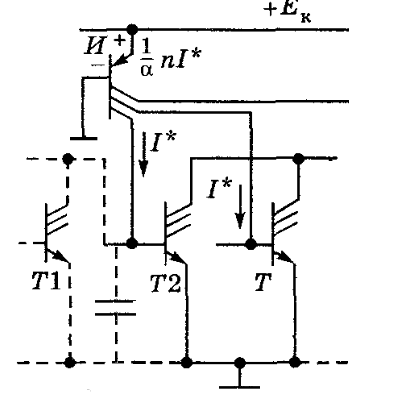
\includegraphics[scale=1.5]{iil/image009.png}}
		\caption{}	
		\label{iil9}
	\end{figure}
\end{center}


Как уже было сказано, напряжение база эмиттер транзисторов VT1 и VT2 в режиме насыщения 0.75В. Это означает, что для перевода транзистора в насыщение и переключения ключа емкость C (показана на рисунке) нужно зарядить до заряда, соответствующего напряжению 0.75В. В частности, q=CU = I*t. (Для разрядки используется ток Ib) Отсюда получается, что быстродействие тем больше, чем больше базовый ток. Значит, для повышения быстродействия нужно увелить ток источника, питающего схему на иил ключе. Но тогда возрастет используемая мощность.




